\section{Detector Installation}
\label{sec:fdsp-tc-inst}

\subsection{Introduction}
\label{sec:fdsp-tc-inst-intro}

The DUNE detector installation will proceed in three phases the CUC setup phase, the installation setup phase, and the detector installation phase. The CUC setup phase is the first step in the installation process. The start of the CUC setup phase begins when the underground area for the North Cavern and Central Cavern become available to LBNF and DUNE. At this time the cryostat construction can begin in The North Cavern and equipment installation can begin in the Central Cavern or the Central Utility Cavern (CUC). The main equipment from DUNE which is installed in this phase is the equipment in the DUNE dataroom. The detector installation setup phase begins during the cryostat membrane installation period. In this phase the equipment needed to perform the detector installation will be erected in North Cavern. This includes the installation of the bridge across the cavern, the installation cleanroom, lifting equipment and work platforms, the cold boxes and cryogenic system for testing APA, and the DSS with related switchyard. In the third phase of the installation the detector itself will be installed. The work in each phase will be described the following sections.

\begin{dunefigure}[Layout of the underground area]{fig:cavern-layout}
  {Top view of the layout at the 4850 level at SURF. Shown are the 3 large excavations and the location of detectors in excavation \#1 and \#3. Excavation \#2 is the CUC which houses the DUNE dataroom and the underground utilities.}
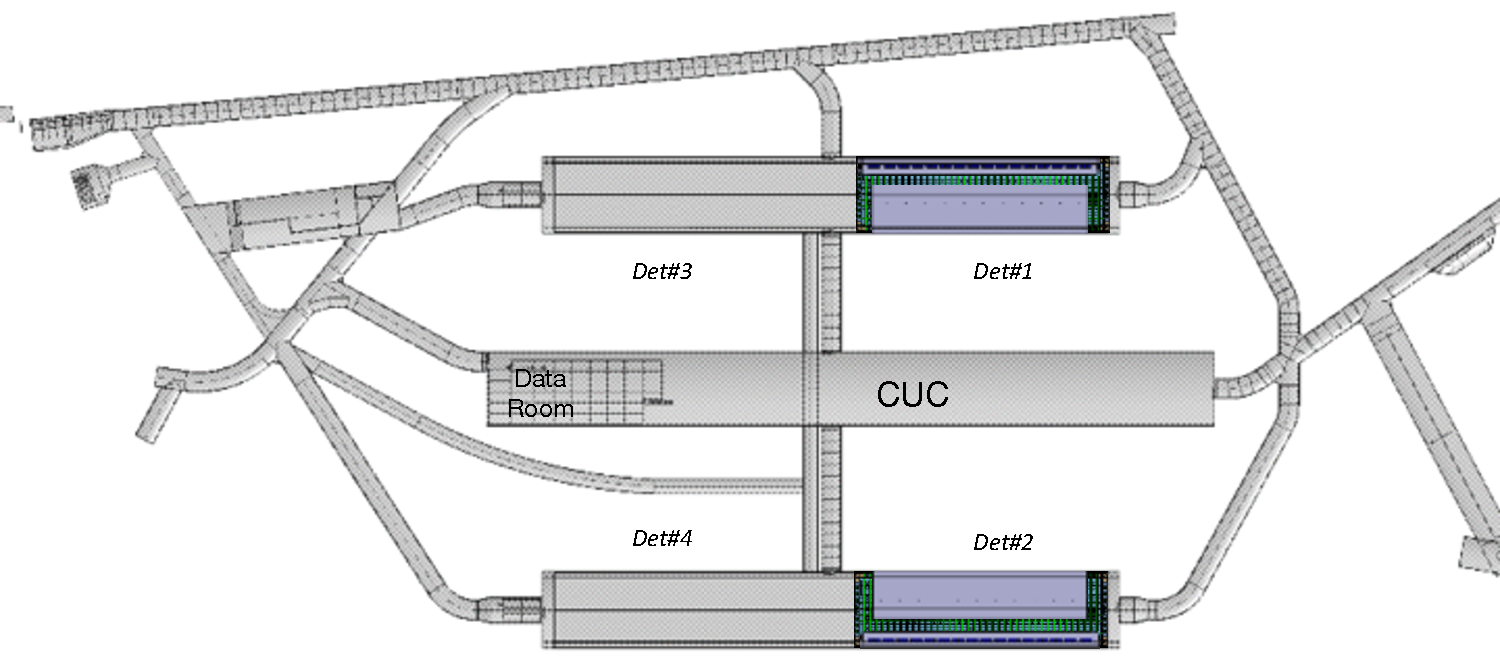
\includegraphics[width=.9\textwidth]{cavern-layout}
\end{dunefigure}

\fixme{insert very simple schedule}

%%%%%%%%%%%%%%%%%%%%%%%%%%%%
\subsection{Installation Process Description}
\label{sec:fdsp-tc-inst-proc}

\subsubsection{CUC Installation Phase}

\begin{dunefigure}[Layout of the DUNE dataroom and experimental workarea in CUC]{fig:install-cuc}
  {TOP: The overall layout of the DUNE spaces in the CUC is shown. The inner room is the DUNE dataroom which houses the underground computing and the outer area referred to as the experimental workarea is a general purpose workarea. Bottom: The first row of racks in the data room is shown. The first two racks are the  CF interface racks. The image was taken from the ARUP design drawing U1-FD-T-701}
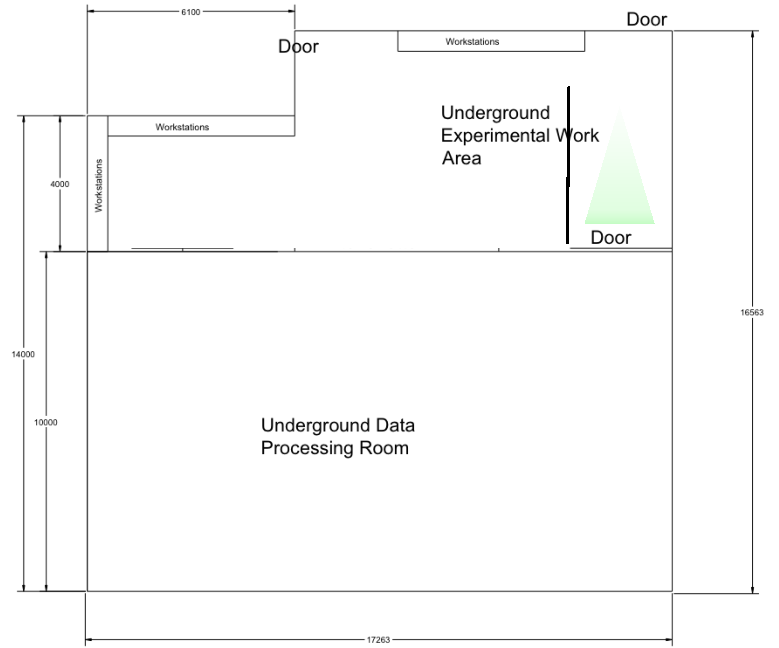
\includegraphics[width=.7\textwidth]{cuc-layout}
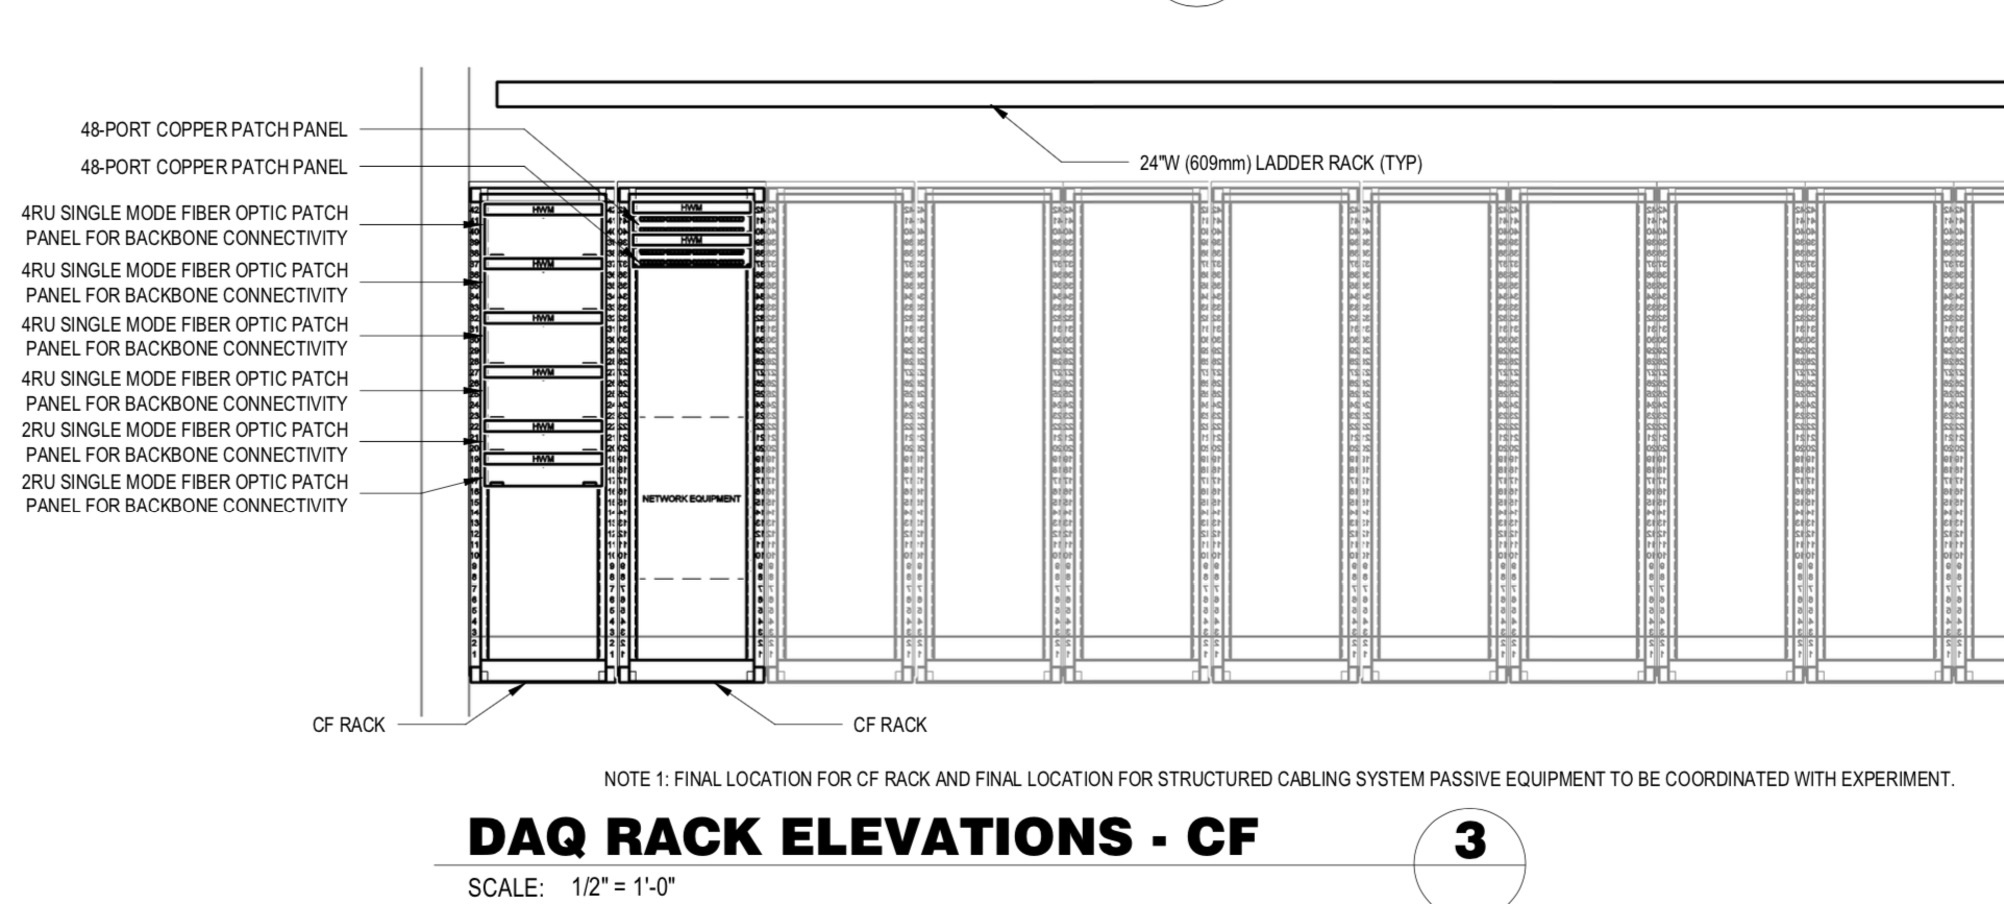
\includegraphics[width=.9\textwidth]{cuc-cf-racks}
\fixme{need to use a figure from the 90\% submittal}
\end{dunefigure}


The first stage of the CF work ends when the outfitting of 
the North and Central caverns is complete. At this time the CUC is ready for DUNE outfitting and the cryostat installation can start for detector 1. During this period DUNE will not have assess to the detector excavations as the heavy steel work for the cryostat will be ongoing. The only work planned for DUNE in this period is the outfitting of the data room and work area room in the CUC shown in Figure \ref{fig:install-cuc}. CF will provide the empty room with an 18 in false floor, a 500KVA power disconnect, and connections for chilled water sufficient to cool the racks. The dataroom like the adjacent CF electronics room will be outfitted with a dry fire extinguishing system. 

The water cooled racks, cable trays, power distribution, and water distribution are the responsibility of DUNE and will be installed once the space becomes available. The installation of the racks needs to be coordinated with CF as the first two racks are for CF usage and need to be in place before the underground phase one work is complete. Some small overlap will be needed between CF and DUNE at this time.

At the same time the eight DAQ racks which receive the data from the underground area and then transmit the data to FNAL will also be installed. With this infrastructure in place the DAQ group can begin constructing and testing the final DUNE DAQ.  

The underground experimental work area is a general purpose area that will need to serve many purposes during the DUNE installation. Initially the area will be outfitted with office equipment for the installation team, workstations for DAQ, and a basic conference area for meetings.  The room is 4-6.4 \si{m} deep and 20 \si{m} long so it can serve several functions.

During this early installation stage the machine shop and DUNE storage area will also be setup in the detector excavation area.

\subsubsection{Installation Setup Phase}

Once the steel structure of the cryostat is complete the remaining work will be focused inside the cryostat. 
There will still be a lot of activity outside the cryostat as the 4,000 crates of foam and other materials are transported inside but the outer structure will be in position so some DUNE work can start. 
The first piece of equipment to installed will be the bridge between the North and South drifts. 
This will allow the cryogenics equipment to travel from the North drift to the CUC and will provide part of the structure for the cleanroom. 
Construction of the cleanroom frame and related hoisting equipment can then begin. 
The largest most complex equipment that must be constructed in this phase are the cold boxes and related cryogenics system. 
Due to the size of the cold boxes these must be constructed in place. 
The layout of the installation region outside the cryostat is shown in Figure \ref{fig:install-ug-layout}. 
This figure shows a cut below the bridge so the majority of the installation equipment can be seen. 
The three 15 \si{m}tall cold boxes are seen in blue next to the yellow access stairway. 

The hoisting equipment and the rail system needed to move the detector components in the installation area interfaces with the bridge, cryostat and possibly the cleanroom mechanical structure. 
Installing this early will make transporting equipment around the area outside the cryostat significantly simpler. 
\fixme{Do we want a figure of just the rails and switchyard?} 
The assembly towers for the APA assembly, APA cabling, and CPA assembly can be installed when it is most convent for the cryostat installation crew. 
Just prior to the start of detector installation the cleanroom walls will be installed, the area will be cleaned and added filters will be installed to convert the area to an ISO-8 cleanroom.

During this phase of the cryostat installation the majority of the cryostat work will be inside an at the 4910 level. 
This will allow significant work to be performed on the cryostat roof for the cryogenic system installation and the detector installation setup. 
The cryostat crossing tubes will be installed on the roof 
\fixme{figure of the cryostat crossing tube with the mechanical connection to the I-beams and the inteface to the membrane.} . 
These assemblies are welded to the 1 \si{cm} thick steel cryostat roof and are then additionally cross braces to the large I-Beams. 
The thick walled tubes which penetrate through the foam insulation are in place at this time. 
Once the crossing tubes are in place the large tees for the cold electronics can be installed. 
The next step in the installation requires the internal roof of the cryostat to be complete. 
At this time the DSS support feedthrus can be installed and possible the DSS beams can be lifted into positions. 
The details of how to coordinate this work will be iterated with the cryostat manufacturers as the design work is completed. 
At this time the cold electronics mechanical feedthrus can be installed. 
Once work on the feedthru are complete then the mezzanines for the cryogenic system and the detector electronics racks can be installed.
Finally the cable trays,  piping, lighting, and cryostat roof flooring are installed. 
At this time the cryostat roof is ready for the start of the DAQ installation in the detector area.

The last steps in the installation setup phase is the installation of the cryostat internal piping, cleaning the cryostat, installing the false floor, and filtered lighting to protect the photon detectors. 
\fixme{ Insert the figure of the piping inside the cryostat. }



\subsubsection{Detector Installation Phase}

\begin{dunefigure}[Top view of the installation region inside the cleanroom ]{fig:install-cleanroom-layout}
  {Top view of the cleanroom used for installation. In this view cleanroom roof and bridge are not shown. The equipment used for the installation is shown along with the material airlock layout and the location of the changing room. The cryostat is to the right of the figure and the I-Beams passing through the TCO opening are shown.}
 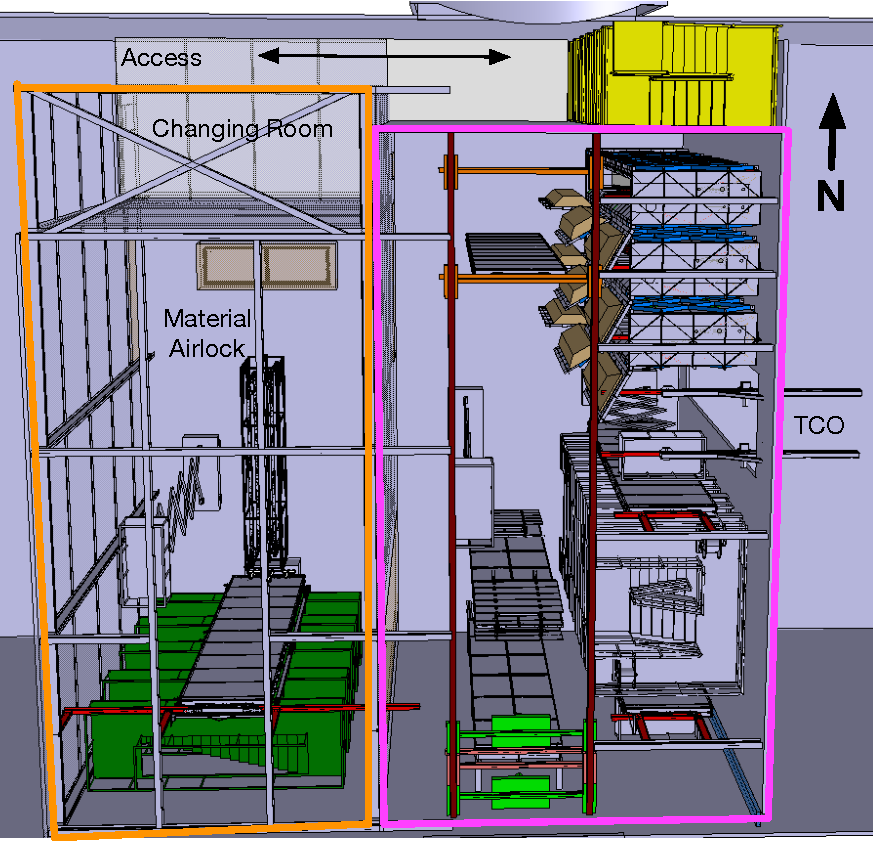
\includegraphics[width=\textwidth]{install-cleanroom-layout}
\end{dunefigure}

At the start of the detector installation phase the work on the cleanroom is complete, the DSS is installed in the cryostat including the switchyard near the TCO. 
The light in the cryostat and cleanroom will be filtered to protect the photon detectors and the air will be filled to reduce the dust collected during installation. 
The cryogenic piping will be in place along with the false floor. 
The false floor both gives a flat work area and protects the 1.2 \si{mm} thick stainless steel cryostat membrane. 

The layout of the cleanroom during the detector installation phase is shown in Figure \ref{fig:install-cleanroom-layout}. This image is a top view of the cleanroom with the roof and bridge removed; the cryostat is on the right and the open cavern on the left. In the North-East corner of the figure the access stairway is shown in yellow. This stairways is outside the cleanroom and allows people to access the 4910 level from the North drift or from the cryostat roof. An access corridor along the north wall connects the stairway to the rest of the cavern. The changing room and airlock are found on the West of the figure and are outlined in orange. The changing room is located in the the North-West corner and provided access to both the cleanroom and the airlock. South of the changing room is the material airlock. This rather large area is where the APA modules are connected together to form the 12 \si{m} tall units. The assembly station is shown in green along the south wall of the airlock. This area is also where all the materials are brought from the dirty outside cavern and are cleaned or the outer packaging removed. Roll-up doors along the West wall allow material from the outer cavern to be brought into the airlock. A section of the roof can be removed to allow the cavern bridge crane to manipulate the APA transport box and modules. The cleanroom area itself is shown on the right of the figure outlined in magenta. Inside the cleanroom is a switchyard material transport system (shown in red) similar to what is used for the DSS inside the cryostat. The switchyard is used to move the assembled detector components north-south in the cleanroom. East-west rail sections are then used to deliver the components to the required work location. In the north area of the cleanroom are the three cold boxes used to cryogenically test the fully assembled and cables APA pairs. In the south half of the cleanroom is the APA cabling tower used for cabling and testing the APA pairs. Along the South wall is the CPA assembly fixture for assembling the CPA. 

\begin{dunefigure}[Endwall hoisting infrastructure]{fig:install-endwall-1}
  {Image showing the hoisting equipment used to lift the Endwall into position. In this image one of the Endwalls is in place and a second is being positioned.}
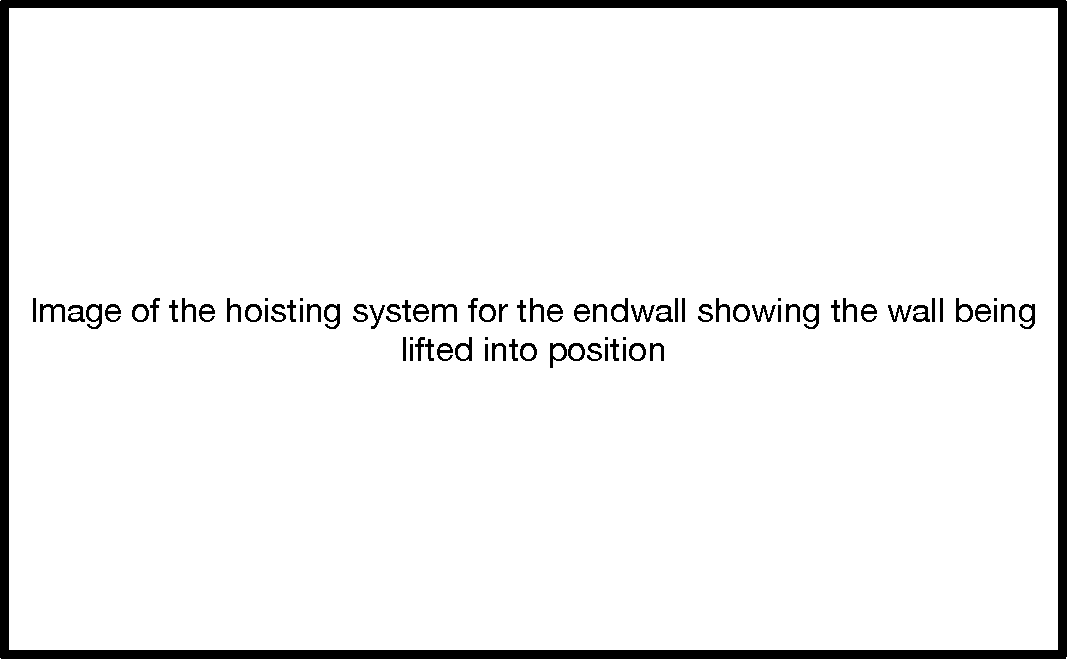
\includegraphics[width=.9\textwidth]{install-endwall-1}
\end{dunefigure}

The first detector equipment to be installed is the CISC thermometers and cameras at the East end of the cryostat which will be used to monitor the cool down, filling and commissioning of the detector. As these components are small the installation work can be performed using a scissor lift with 12 \si{m} reach. 
At present this is the tallest battery operated (thus cleanroom compatible) scissor lift rated for use in the US that we have identified.

The next step in detector installation is the field cage end-wall installation. 
The end-wall panels will be brought underground in custom crates as slung loads. 
Each of the 8 crates will hold 4 end-wall sub-panels and 8 sub-panels are needed to build one complete 12 \si{m} tall panel.  
The first step in the end-wall installation is to install a custom hoist to the end of the DSS beam. 
This will be used to lift and assemble the sub-panels in place. 
The end-wall transport crates will then be brought to the material airlock using a forklift where they are either un--crated or the crates are cleaned. 
Once clean the crates are moved into the cleanroom and placed next to the TCO. The a hoist running on the rails through the TCO is used to lift the endwalls into the cryostat.
Inside the cryostat the end-wall crates are moved into position using custom carts or simple pallet jacks.
The top Endwall sub-panel is then attached to the installation hoist and lifted out of the crate. When the sub-panel is free of the crate the cart is adjusted so the second sub-panel can be attached to the first and the pair are then again lifted. This process is repeated until the full 12 \si{m} Endwall field cage panel is assembles and can be attached to the DSS. 
Figure \ref{fig:install-endwall-1} shows an Endwall panel being lifted into position.
At this time all the HV connections inside the panel can be tested. The process is repeated for the four Endwall panels making up the East Endwall. 
In parallel to the endwall installation the cleanroom is configured for the installation of the APA and Cathode plane systems.

\begin{dunefigure}[Installation of the first Endwall]{fig:install-endwall-2}
  {The Endwalls are lifted out of the transport crates using the installation hoist. One panel is lifted then the next one is attached to the bottom. This is repeated until all eight panels are suspended from the installation hoist and then the panels are connected to the DSS.}
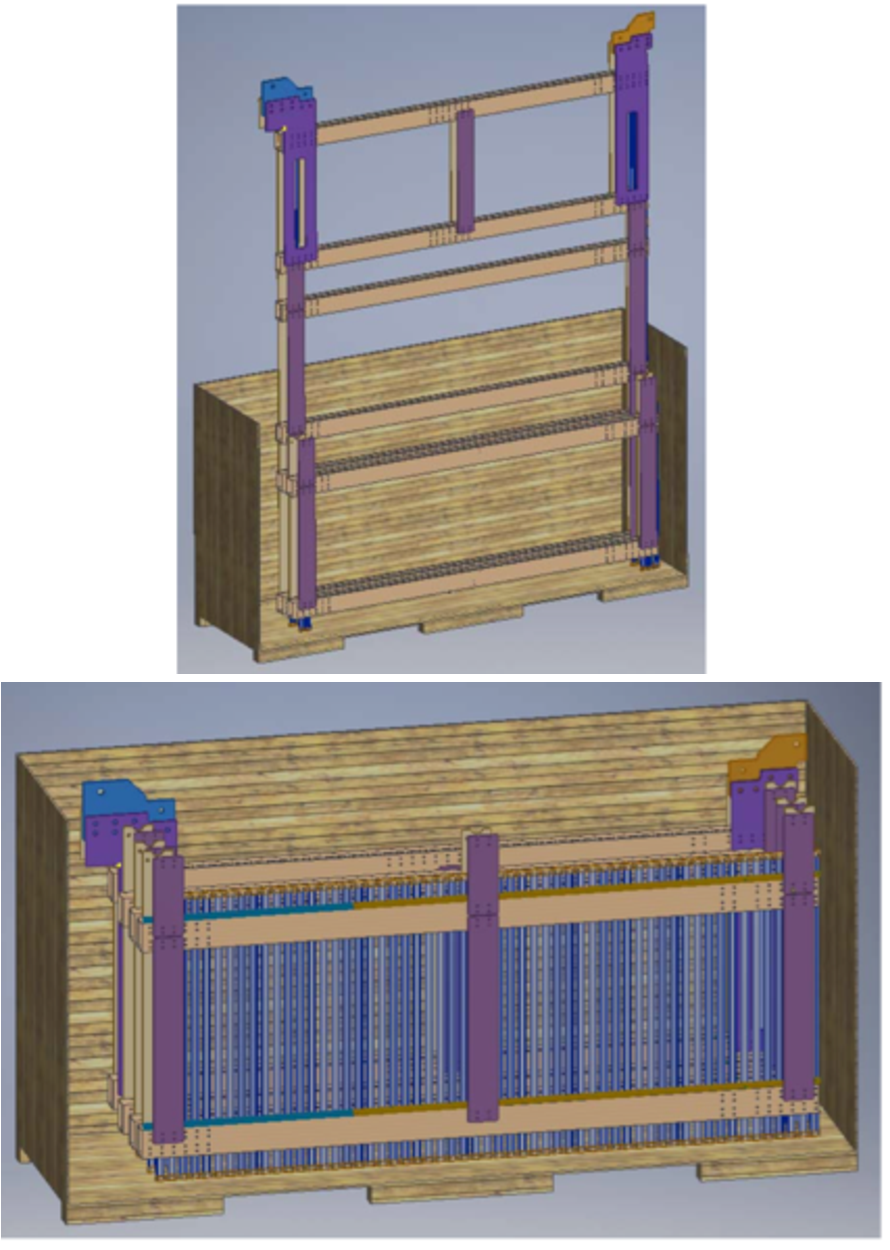
\includegraphics[width=.9\textwidth]{install-endwall-2}
\end{dunefigure}


The installation of the APA and Cathode with Top/Bottom Field cage modules is the most labor intensive period of the detector installation. If possible DUNE would like to finish installing one row of the APA, CPA, and FC modules every week. This represents the equipment shown in Figure \ref{fig:install-single-row}. To achieve this several separate teams will need to be working inside the cryostat positioning the equipment, connecting the cables, and deploying the field cages, while  other separate teams will be working in the outside cleanroom assembling the equipment and performing the final cold tests. The total time that would be needed to install a row of APA and CPA if all the work were to be done serially would be many weeks so performing the work as parallel  as possible will be very important for executing the installation efficiently. 


\begin{dunefigure}[Single row of APA and CPA]{fig:install-single-row}
{One row of the APA and CPA with associated field cages is shown. In this  image the field cages are deployed in the final orientation. The equipment in the figure represents $1/25$ of the total TPC.}
 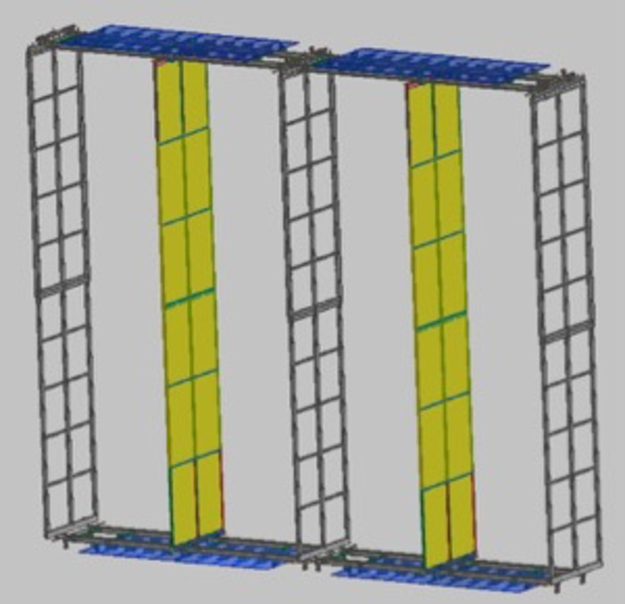
\includegraphics[width=0.5\textwidth]{install-single-row}
\end{dunefigure}

When the APAs are installed the area outside the cleanroom in the North cavern is available for storage and and it has capacity to store one full month of equipment. Equipment will be brought into the cleanroom's materials airlock through a rollup door in the West wall using either an electric forklift or electric pallet jacks.  The APAs enters the airlock in the transport crates which were used to bring the APAs down the Ross shaft and into the North cavern. Each transport box hold two APA with associated electronics and photon detectors and they enter the airlock in a horizontal or "landscape" orientation. Once inside the airlock the dirty outer panels of the transport box are removed, a section of the roof is opened and the bridge crane is used to lift the transport box into vertical. The airlock can then be cleaned and prepared for the APA assembly step where the upper and lower APA are assembled into a 12 \si{m} tall pair. The APA assembly sequence is shown in Figure \ref{fig:apa-assembly-v3}.


After initial visual inspection the lower APA is lifted out of the transport box again using the bridge crane and mounted on the APA assembly tower shown in green on the top row of images in in the Figure \ref{fig:apa-assembly-v3}. The  lower APA is supported from the bottom and guides connected to the sides of the APA provide mechanical stability while allowing the APA to be lifted using jacks integrated into the lower support. Next the upper APA is lifted out of the transport box and the transport box is removed from the airlock. The upper APA is connected to the transport rail above the APA assembly tower. At this point the upper APA is supported by the trolleys used for moving the APAs along the transport rails and it is stabilized using the APA assembly frame. The bridge crane is no longer needed after this step so airlock roof can be closed allowing the air to be purified. In order to assemble the two APA a metal linkage with electrical isolators is inserted into the upper APA and bolted into place. Then the lower APA is raised until the linkage can be bolted to the lower APA.  The APA pair can then be released from the assembly tower supports and jacks and is supported from the top APA to the rail system.
After the air quality in the airlock meets the requirements for ISO-8 and any dust covers are removed from the APA pair the APA can be moved into the cleanroom through a narrow vertical door in the cleanroom wall shown in brown in the top row of images in Figure \ref{fig:apa-assembly-v3}.


\begin{dunefigure}[APA assembly steps]{fig:apa-assembly-v3}
  {Top row from left:  \dword{apa} transport crate inside the airlock; \dword{apa} transport crate rotating to vertical position;  lower \dword{apa} placed on the \dword{apa} assembly frame; and upper \dword{apa} placed on the assembly frame. Bottom row right to left: \dword{apa} pair moving on the cleanroom transport rails; \dword{apa} in  position at the cabling tower; and the \dword{apa} being inserted into the coldbox.}
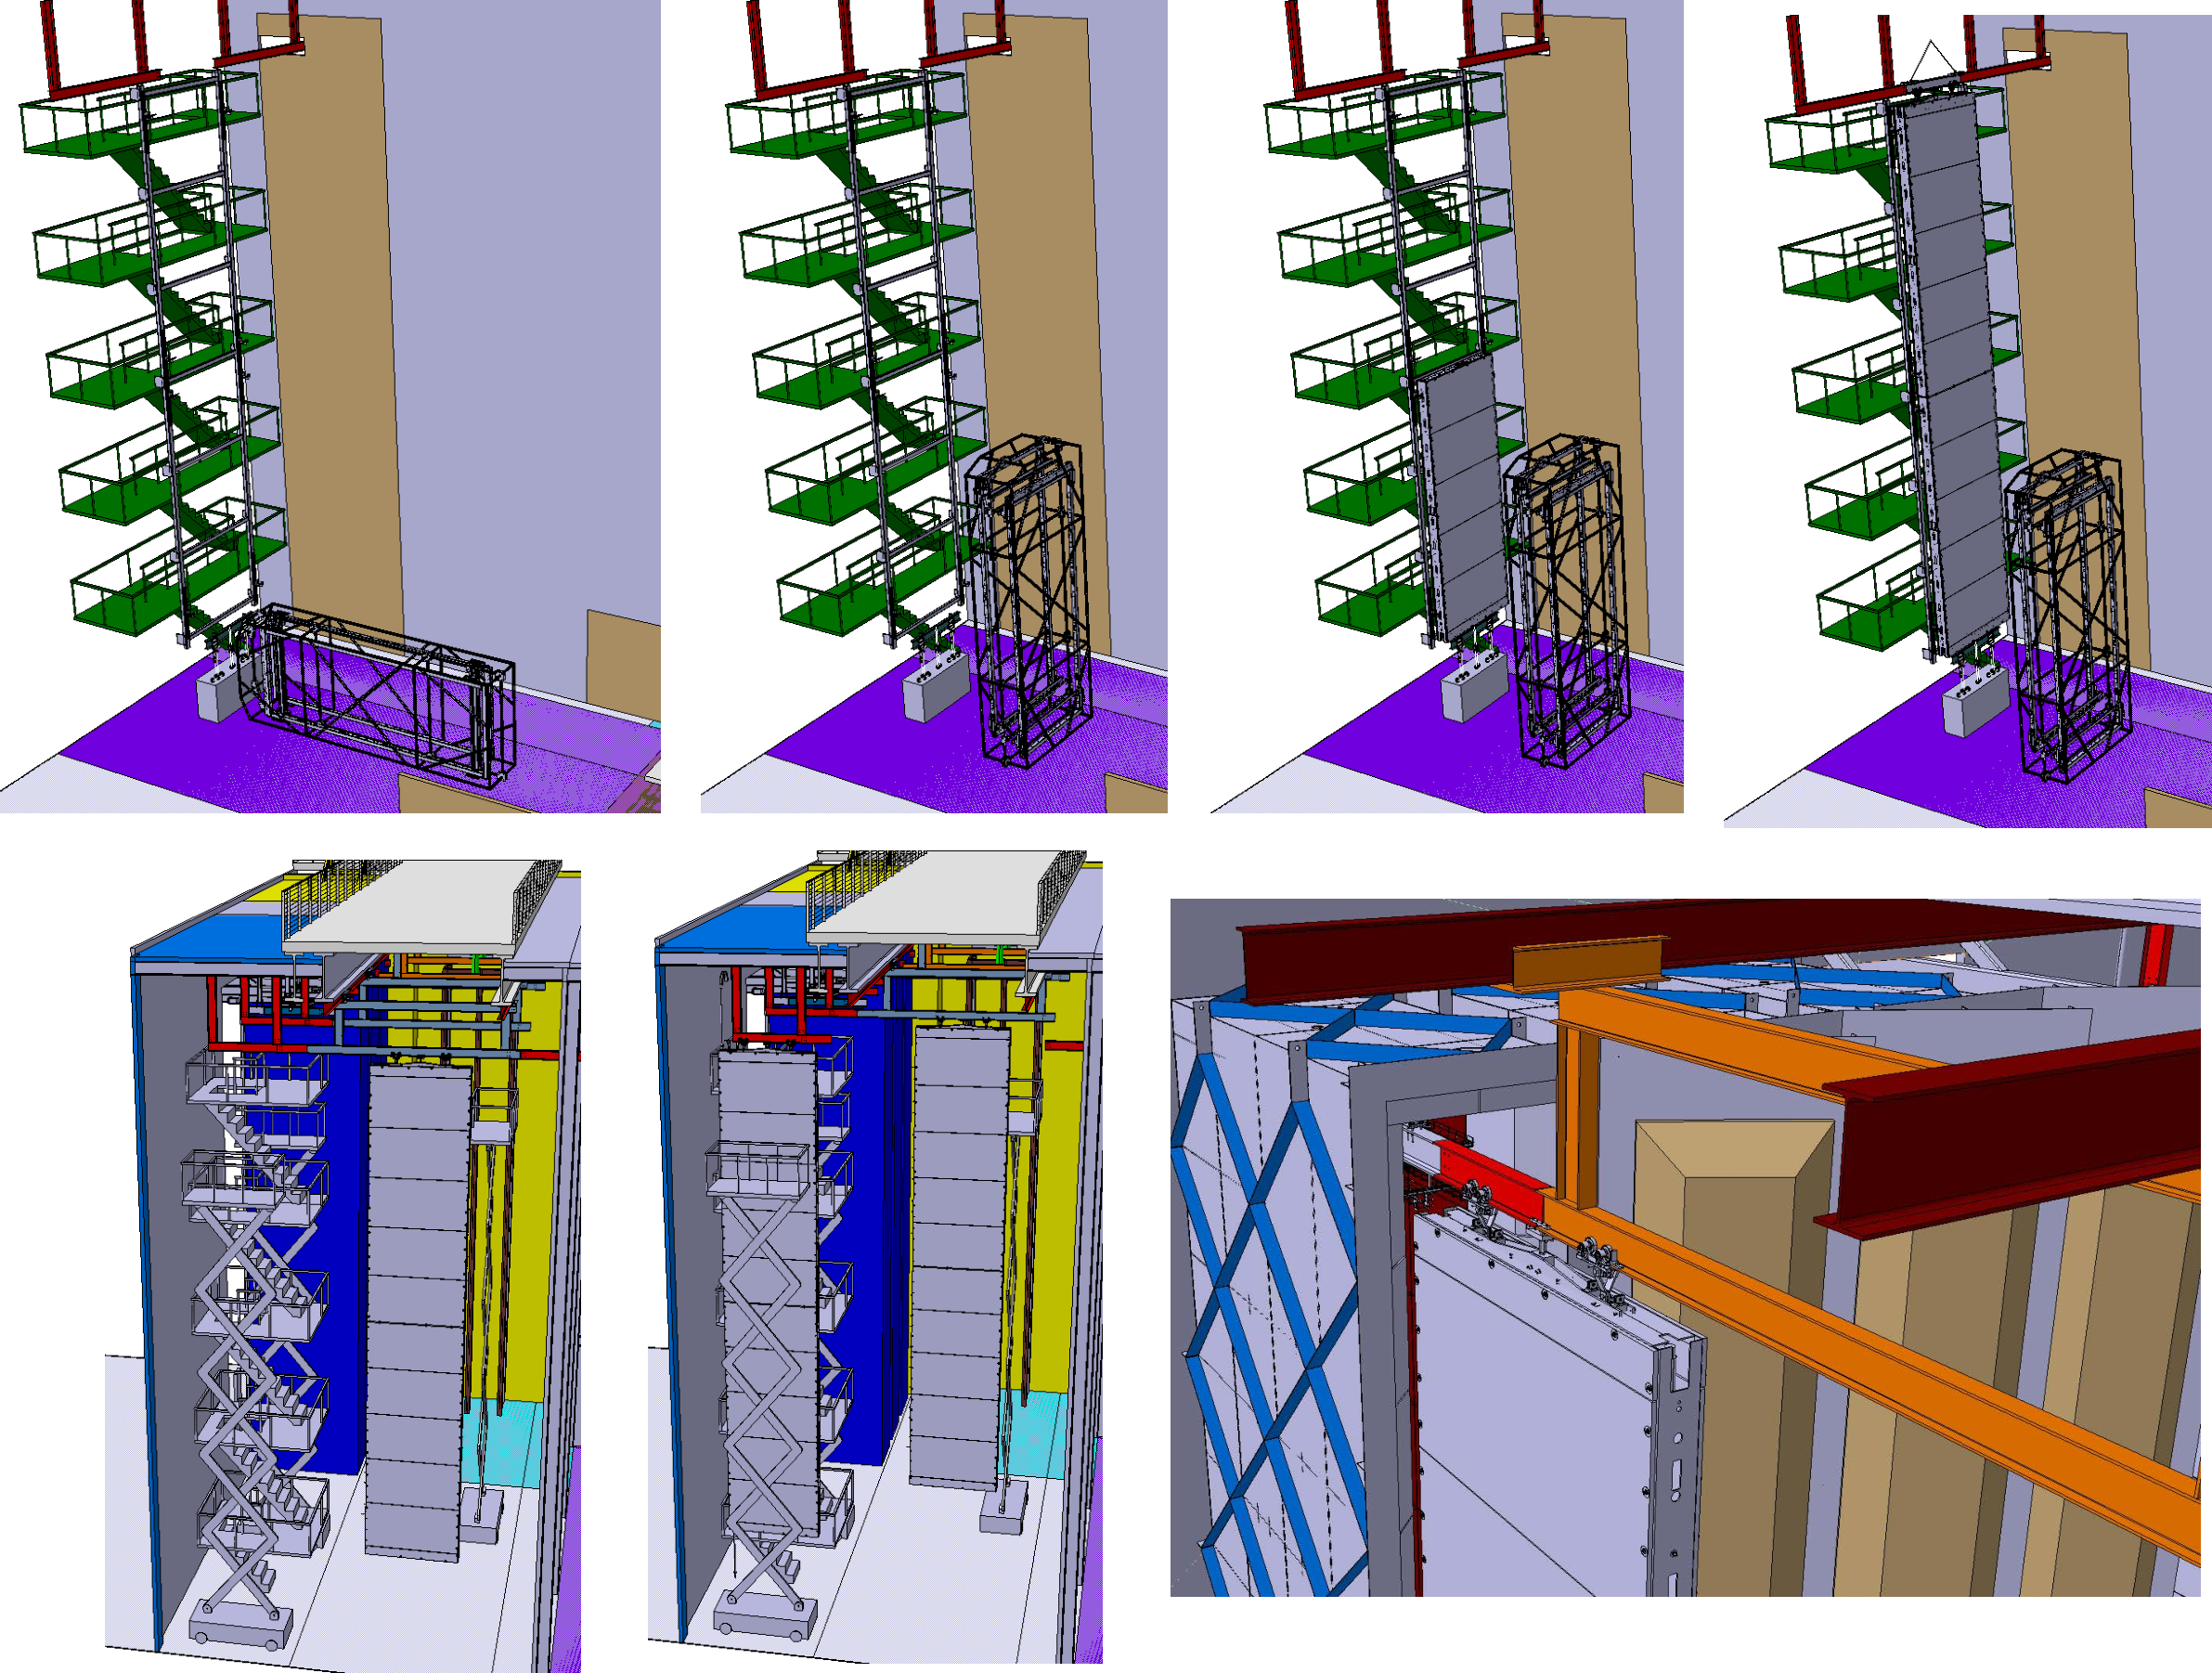
\includegraphics[width=.9\textwidth]{apa-assembly-v3}

\end{dunefigure}

The APA pair moves onto one of the shuttle beams in the cleanroom switchyard and can be moved north-south inside the cleanroom. The next assembly step is to install and test the electronics cabling. The APA is moved to line up with one of rails used to transport the APAs to the APA cabling tower. The lower left two image in Figure \ref{fig:apa-assembly-v3} shows the APA cabling tower in the cleanroom and an APA being moved into position. The APA cabling tower is capable of holding two APA pairs simultaneously allowing one APA pair to be cabled while a second APA undergoes electrical testing in parallel. In this position the cable trays and any other equipment needed during the cabling process can be installed. The electronics cables are delivered to the cleanroom on reels pre-bundled and tested. A lower APA reel is craned up to the top of the APA cabling tower and the cable is then spooled over to a motorized deployment spool and the cable guide is attached. The cable guide is then fed through a guide sieve and into the conduit on the side of the APA. The cable bundle is careful fed through the conduit and is anchored in place using a cryogenic compatible cable grip. The cable connected to the electronics at the bottom and is laid into the cable trays on top. This process is repeated for the second lower APA cable bundle. Finally the upper cables can be installed and prepared for transport. At this time a check of the functionality of all the electronics is performed. After the APA electrical test the APA pair is transported to a cold box where it undergoes a thermal cycle and complete system test. The APA being inserted into the coldbox is shown in the lower right image in Figure \ref{fig:apa-assembly-v3}. As the cold box is also a Faraday cage noise levels can be measure and the photon system checked for photon sensitivity. After the cold test is complete an APA will either move back to the cabling station if any repair is needed or it will be moved into the cryostat for installation. 



\begin{dunefigure}[CPA assembly steps]{fig:install-cpa-assembly}
  {The \dword{cpa} assembly steps are shown. Top row from left:  \dword{cpa} are delivered to the CPA assembly fixture in the cleanroom, the 3 \si{m} sub-panels are lifted onto the frame and connected. Bottom Row: After the CPA panel is complete it is moved into the room and the field cage modules are attached. The CPA is then moved into the cryostat.}
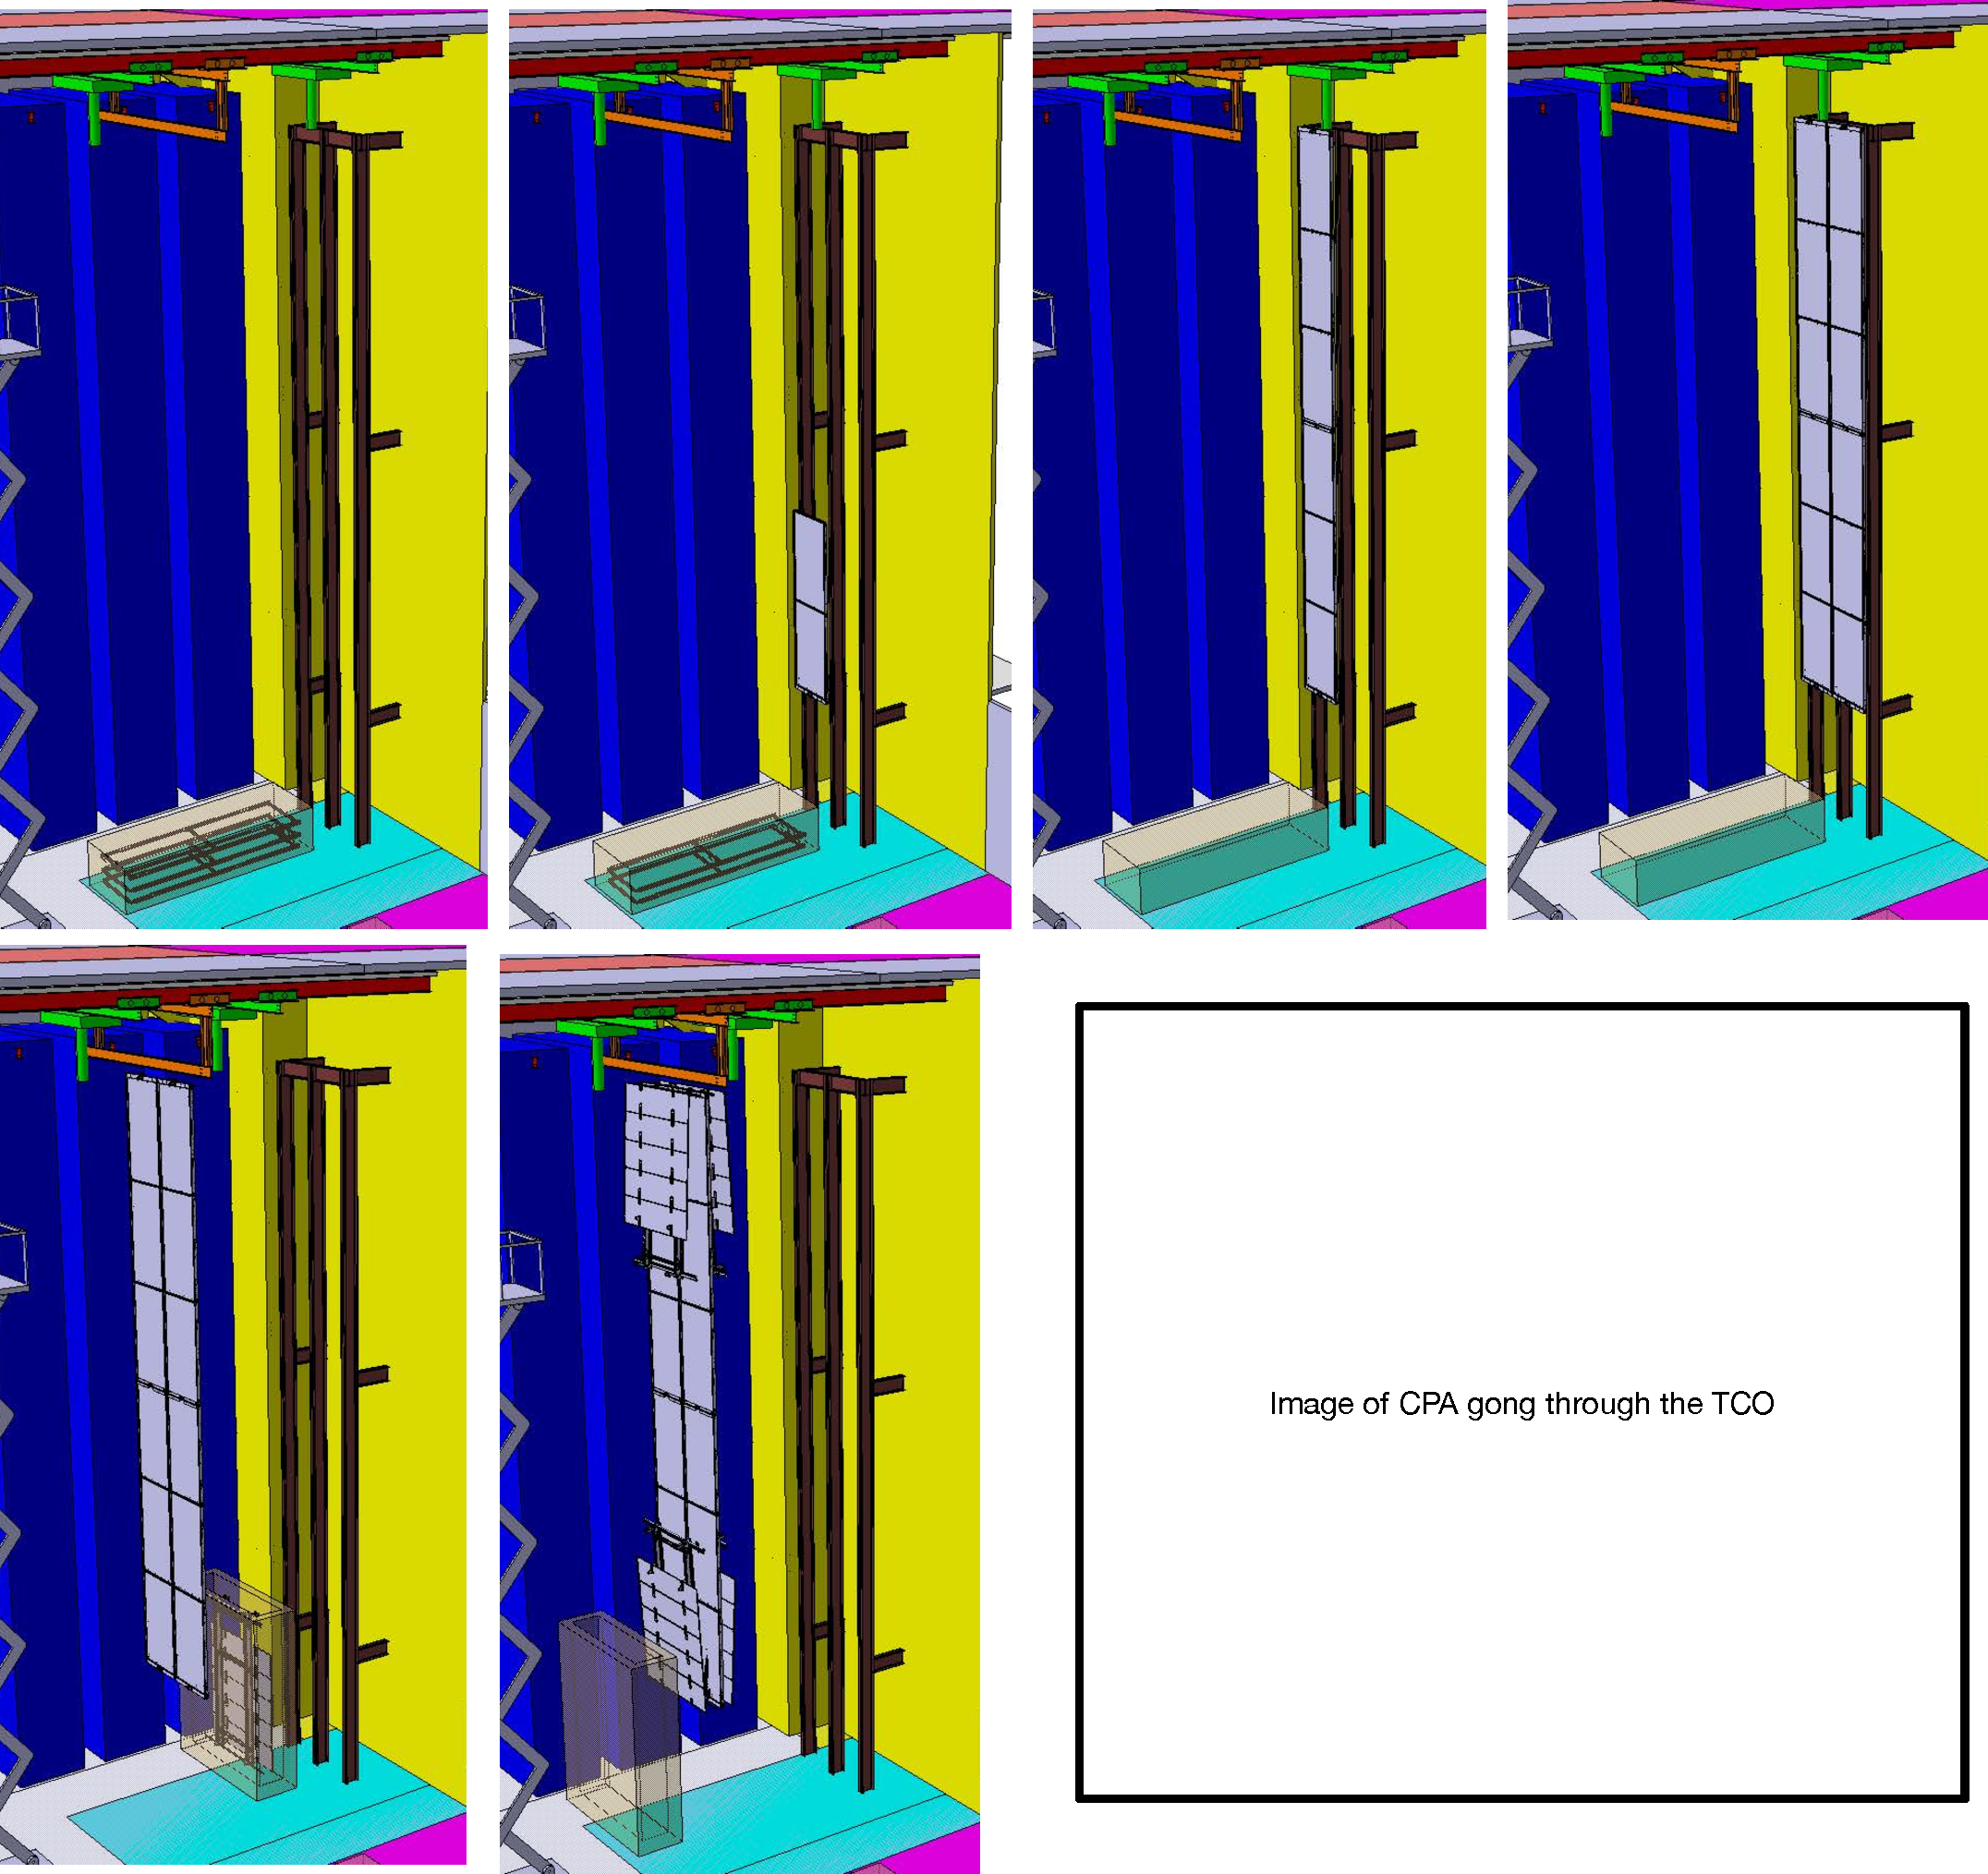
\includegraphics[width=.9\textwidth]{install-cpa-assemble}
\end{dunefigure}

The CPA and top/bottom field-cage modules are assembled in parallel to the APA assembly. Figure \ref{fig:install-cpa-assembly} shows the  assembly sequence. The sub-panels for the cathode plane are delivered to the airlock in crates which hold 3 \si{m} long 1.15 \si{m} segments. The crates after cleaning are brought into the cleanroom and opened. The panels inside are bagged to provide additional dust protection. The sub-panels are lifted out of the crate and place on the assembly frame using the cleanroom switchyard hoist. First one of the 1.15 \si{m} 3 
\si{m} tall sections are assembled and then the second one. Once the 2.3 \si{m} by 12\si{m} assembly is complete the assembly can be connected to the overhead rails with the support rods and trolleys. The assembled cathode panel is then moved away from the wall and the top field cage modules are attached. In Figure \ref{fig:install-cpa-assembly} the completed assembly is show with the lower field cage modules also attached. This is an option but present planning is to install the lower FC modules  inside the cryostat. Finally the CPA-FC assembly is moved into the cryostat.





Work inside the cryostat will proceed in parallel to the work in the outer cleanroom. 
The large detector components like APA pairs and CPA modules will enter the cryostat using the TCO rails which connect to the DSS switchyard.
Inside the cryostat the modules will be pushed onto one of the switchyard shuttle beams shown in  Figure \ref{fig:shuttle}. 
The DSS shuttle beam is then moved to the appropriate row of the DSS and then the module is pushed down the length of the cryostat into position. The position of the DSS beams are well defined and accurately surveyed so the APA and CPA modules can be accurately located by precisely positioning them along the DSS beams. A small correction in the height of the modules may be needed to accommodate deflections in the DSS due to load. Figure \ref{fig:install-ce-cables} shows the typical situation during the APA installation and cold electronics cabling. 

\begin{dunefigure}[Cold Electronics cabling inside the cryostat]{fig:install-ce-cables}
  {The installation of the APA and cabling of the cold electronics is described. In the left panel the situation is shown during the APA installation process. One row of APA and HV equipment is installed and a second APA is ready for the electrical cabling. In the top right image the cable trays are seen which will hold the CE cables and one of the workers in the scissor lift. In the left bottom image thework space is defined wiht the geometry of the APA the cryostat roof and the cable feedthru.}
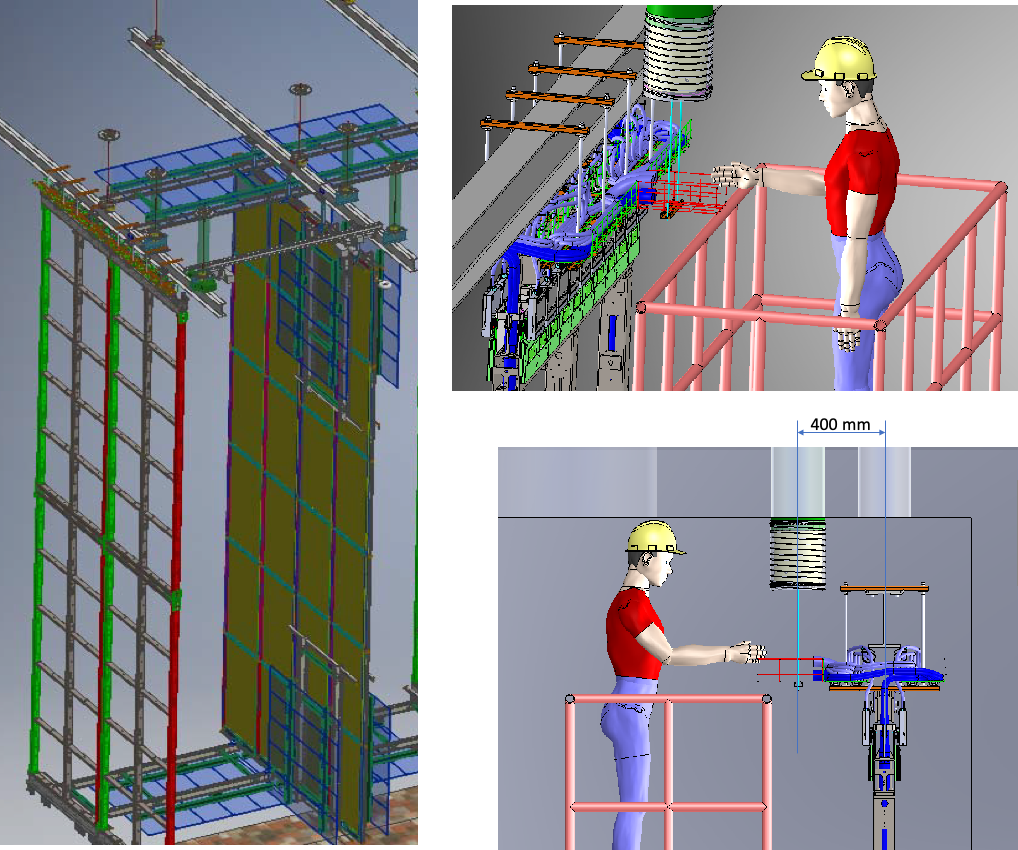
\includegraphics[width=.9\textwidth]{install-ce-cables}
\end{dunefigure}

After the APA is moved into position the permanent support rod is connected to the DSS beam and the trolleys are removed. The crawler used to push the APA along the rails is then moved back through the shuttle area and can be used for the next module. After the APA is locked in position the CE cabling can start. Even if a CPA module is already in position there is over 3 \si{m} space free between the APA and CPA so a scissor lift can easily be positioned in front to the APA. The two right images in Figure \ref{fig:install-ce-cables} show the situation at the top of the cryostat at during the cabling period. The cables are not shown so one can see the cable trays and their support infrastructure. At the start of the cabling all the cables are in the cable trays. A team of two people are in the scissor lift in front of the APA and  and a team of two people are on top of the cryostat. The cables from the bottom APA emerge from the side APA side-tube and are split into two bundles in the cable tray for a total of 4 cable bundles. The top APA also has the cables organized into 4 bundles. During the cabling process each bundle is partially removed from the cable tray and then fed up through the cable feedthru. At the top of the feedthru the cables are strain relieved and then the cables are strain releived again at the bottom of the crossing tube. This is repeated for each of the 8 cable bundles needed for the APA pair. When all the cable are installed through the cable tray Any excess length is returned to the cable tray at the top of the APA. On the roof the short individual cables are then connected to the feedthru flange and the electronics can be tested. When all the electronics and electrical connections are good the flange connecting the warm interface crate and can be sealed to the cryostat feedthru flange and the cable installation is complete. The electronics for each APA is continuously monitored after installation. 

\begin{dunefigure}[CPA assembly steps]{fig:install-cpa-fieldcage}
  {The steps to deploy the field cage modules after the \dword{cpa} is in position are shown. The field cage deployment tool is mounted above the DSS beams and a cable is connected to the top field cage module. The module is then lifted into position and latches to the APA module. The bottom APA is lowered using a wheeled cart that connects to the module with a rope. The module is then lowered using a pulley that is free to move on a slide and a winch.}
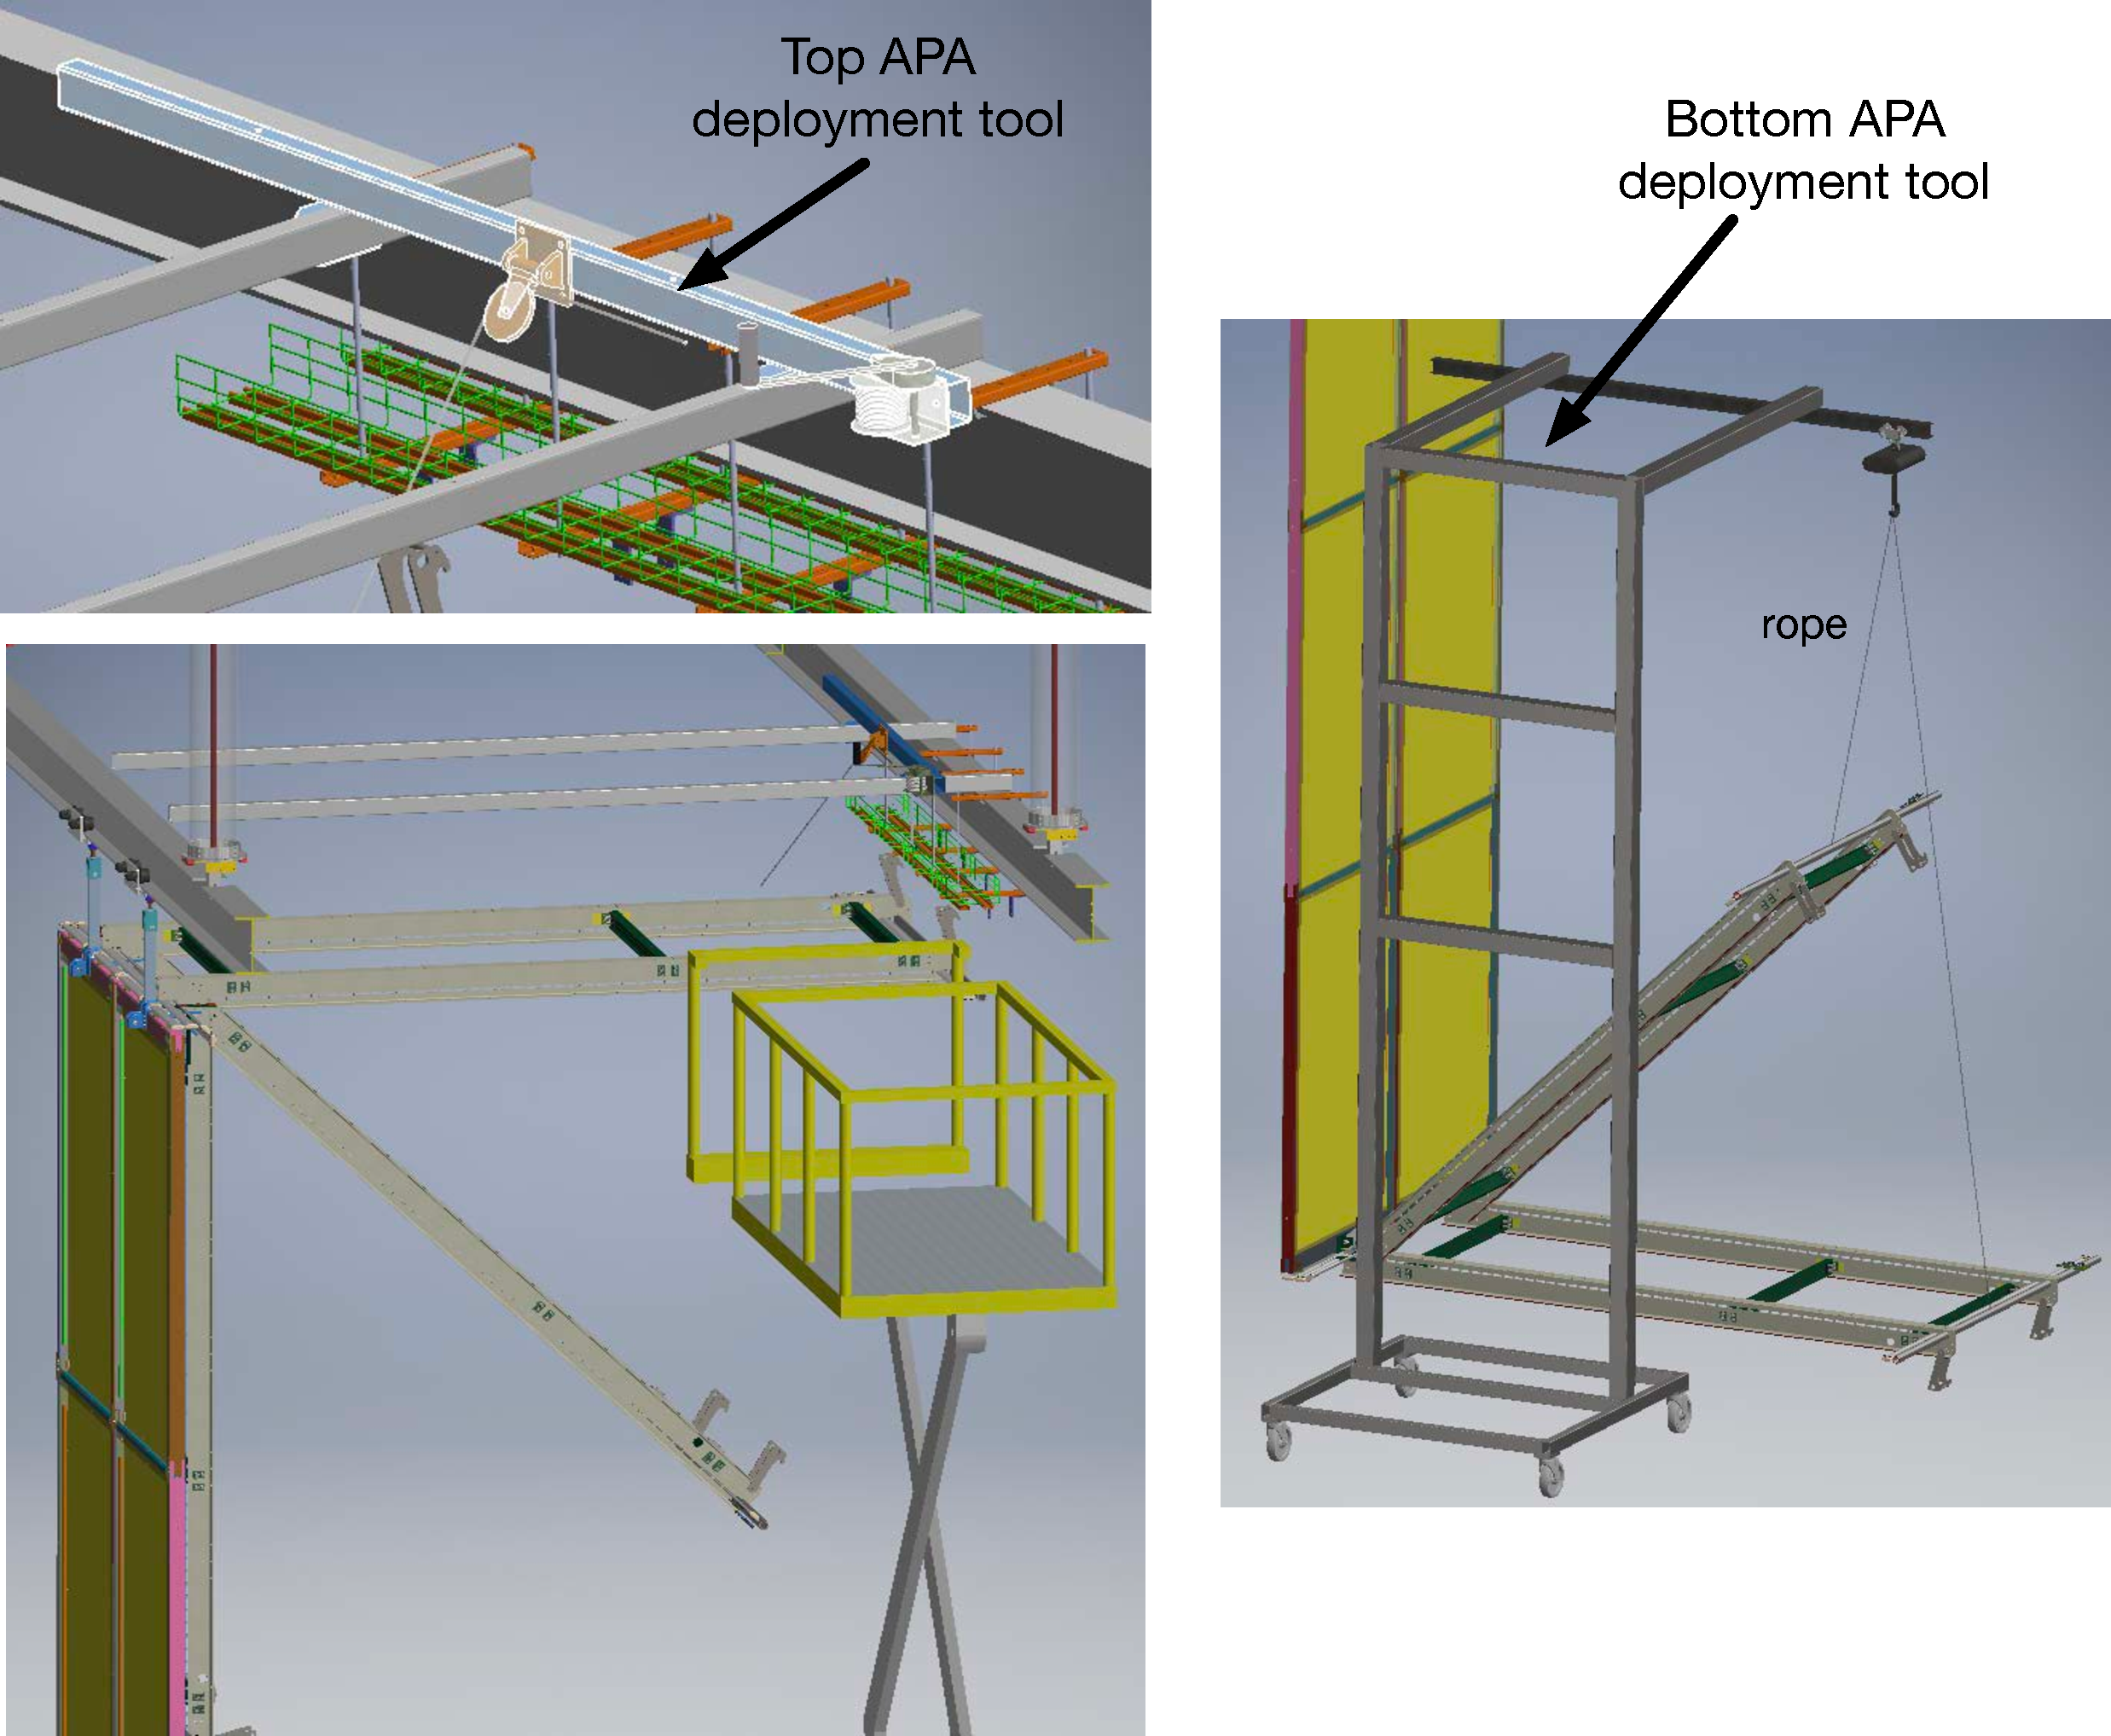
\includegraphics[width=.9\textwidth]{install-cpa-fieldcage}
\end{dunefigure}






% clear the figure buffer before starting the next session
\clearpage

\subsection{Detector Commissioning Phase}
\label{sec:fdsp-tc-inst-comiss}
After the \dwords{detmodule} is installed in the cryostat there remains a lot of work before it can be operated. 
First the \dword{tco} must be closed. 
This requires bringing back the cryostat manufacturer. 
First the missing panel with the steel beams and steel panel are installed to complete the cryostat's outer structural hull. 
Then the remaining foam blocks and membrane panels
are installed from the inside using the roof access holes 
to enter the cryostat. 

In parallel, the \lar pumps are installed at the ends of the cryostat and final connections are made to the recirculation plant. 
Once the pumps are installed, the cryostat is closed, and everything is leak tested, the cryogenics plant can be brought into operation. 
First the air inside the cryostat is purged by injecting pure argon gas at the bottom  at a rate such that the cryostat volume is filled uniformly but faster than the diffusion
rate. 
This produces a column of argon gas that rises through the volume and sweeps out the air. 
This process is referred to as the \textit{piston purge}. 
When the piston purge is complete the cool-down of the \dword{detmodule} can begin. 
Misting nozzles inject a liquid-gas mix into the cryostat
that cools the detector components at a controlled rate. 

Once the detector is cold the filling process can begin. 
Liquid argon stored at the surface  at \surf is vaporized and brought down the shaft in gaseous form and is then re-condensed underground. 
The \lar then flows through filters to remove any H$_2$O or O$_2$ and flows into the cryostat.
Given the very large volume of the cryostat and the limited cooling power for re-condensing, it is  expected to take \num{12} months to fill the first \dword{detmodule}. 
During this time the detector readout electronics will be on monitoring the status of the detector. 
Once the \dword{detmodule} is full, the drift high voltage can be carefully ramped up and data taking can begin.






\fixme{IDR text follows}




















\begin{dunefigure}[APA and CPA installation steps]{fig:Install-seq}
  {Top row from left:  crated \dword{apa} rotating to vertical position;  crated vertical \dword{apa} placed in cart; \dword{apa} panels moved to fixture using the under-bridge crane. Bottom row: series showing \dword{cpa} panels uncrated and moved to fixture. }
%\includegraphics[width=.9\textwidth]{apa-install-seq-top}
%\includegraphics[width=.9\textwidth]{cpa-install-seq-bot}
\end{dunefigure}

\begin{dunefigure}[\dword{cpa} and \dword{fc} unpacking and assembly]{fig:cpa-fc-unpack-assy}
  {On the left, the assembled \dword{cpa} panel is placed onto the north \dword{tco} beam. On the right, the (green) \dword{fc} panels (already lowered into \dword{sas} and moved into the clean room) are installed as the \dword{cpa} array hangs under the \dword{tco} beam. }
%\includegraphics[width=.9\textwidth]{cpa-fc-unpack-assy}
\end{dunefigure}

\begin{dunefigure}[\threed model of underground area showing installation infrastructure]{fig:Install-ISO-Top}
  {\threed model of the underground area showing the infrastructure to install the \dword{spmod} in cryostat~1. The most significant features are presented including the \dword{apa} and \dword{cpa} assembly areas, the region around the \dword{tco} for materials entering the cryostat,  the changing room, the region for the materials air lock, (\dword{sas}), 
  and the means of egress.}
%\includegraphics[width=.9\textwidth]{Install-ISO-Top}
\end{dunefigure}

\begin{dunefigure}[Section view of the \threed model showing layout]{fig:Install-TopView}
  {Section view of the \threed model showing layout, looking down on the installation area from below the bridge. Areas shown, left to right,  are the cryostat and \dword{tco}, the platform in front of the \dword{tco}, the dressing area, the \dword{apa} and \dword{cpa} assembly area (directly under the bridge), and the stairs and elevator. The lower right corner of the region is used as the materials air lock.}
%\includegraphics[width=.9\textwidth]{Install-TopView}
\end{dunefigure}





%The current installation plan is described. 
In the current installation plan, \dword{dune} will take
ownership of the different underground areas at different times. The
surface data room and the underground room in the \dword{cuc} are available
significantly before the collaboration has access to the cryostats; 
the optical fibers between the surface and underground will be in
place even earlier. This will allow a \dword{daq} prototype to be developed
and tested early. The installation of the \dword{daq} hardware can also be
finished before the start of detector installation if desired, so the
\dword{daq} will not be on the critical path.  When the collaboration receives
access to Cryostat~1 the steel work for Cryostat~2 will be
finished and the work on installing the membrane will have
started. Excavation will be complete.  For planning purposes it is
assumed that the first \dword{detmodule} will be \dword{sp} and the second
\dword{dp}. The first step in the \dword{sp} installation is to
install the cryogenics piping and the \dword{dss}. As this piping will
require welding and grinding, it is a dirty process and must be
complete before the area can be used as a clean room. When this is
complete the cryostat can be cleaned and the false floor
re-installed. The clean infrastructure for installing the \dword{detmodule},
including the clean room, work platforms, scaffolding, the
fixturing to hold the detector elements during assembly, and all the
lifts need to be set up. Once the infrastructure is in place and the
area is clean, the installation of the main elements can start. The
general layout of the installation area showing the necessary space
and equipment is shown in Figure~\ref{fig:Install-seq}. 

The \dword{spmod}  is installed by first installing the west endwall or
endwall~1 (see Figure~\ref{fig:endwall}).

\begin{dunefigure}[End view of \dword{spmod} with \dword{ewfc} in
  place]{fig:endwall}
  {End view of \dword{spmod} with \dword{ewfc} in
  place, with one row of \dwords{apa} and \dwords{cpa}.}
%\includegraphics[width=0.6\textwidth]{endwall.png}
\end{dunefigure}

The \dwords{apa} and \dwords{cpa} with top and bottom \dword{fc} panels are
installed next. The plan is to install six \dwords{apa} and four
\dwords{cpa} per week, which is enough to complete one of the \num{25}
rows every week. Additional time is built into the schedule to take
into account that the installation will be slower at the beginning and
some re-work may be needed. By building west-to-east, complete rows can
be finished and tested before moving to the next row. This reduces the
risk of finding a fault after final \dword{fc} deployment and cabling,
which would require dismantling part of the \dword{detmodule}. Some of the steps
needed to install the \dword{apa} and \dword{cpa} modules outside the
cryostat are also shown in Figure~\ref{fig:Install-seq}.  The middle three
panels show how the \dword{apa} needs to be handled in order to rotate
it and mount it to the assembly frame. After two \dwords{apa} are
mounted on top of each other, the cabling for the lower \dwords{apa}, and the
\dword{ce} and \dword{pd} cables can be installed. The
lower three panels show how the \SI{2}{m} \dword{cpa} sub-panels are
removed form the transport crates and assembled on a holding frame. Once
the \dword{cpa} module is assembled the \dword{fc} units can be
mounted. Finally, once the \dwords{apa} and \dwords{cpa} are installed,
the endwall~2 can be installed. A high-level summary of the schedule
is shown in Figure~\ref{fig:Install-Schedule}.

\begin{dunefigure}[High-level installation schedule]{fig:Install-Schedule}
  {High-level installation schedule.}
 %\includegraphics[width=\textwidth]{TP-Schedule-Feb2018.pdf}
\end{dunefigure}






For the \dwords{detmodule} to be installed in safe and efficient
manner, the efforts of the individual consortia must be coordinated
such that the installation is planned as a coherent process. The
interfaces between the individual components must be understood
and the spaces required for the installation process planned and
documented. The installation planning must take into account the
plans and scope of the \dword{lbnf} effort and the individual plans of
the nine consortia. By working with the \dword{lbnf} team and the
members of the consortia responsible for building and installing their
components, a joint installation plan and schedule, taking into account
all activities and needs of all stakeholders, can be developed. Although
the organization of the installation effort is still evolving, 
an installation coordinator will be the equivalent of a scientific lead for this effort.

One of the primary early responsibilities of the \dword{uit} is to
develop and maintain the \dword{dune} installation plan and the
installation schedule. This installation plan 
describes the installation process in sufficient detail to demonstrate
how all the individual consortium installation plans mesh and it 
gives an overview of the installation process. The installation plan
is used by the \dword{uit} to define the underground infrastructure
needed for detector installation and the interfaces it has with respect  to 
the consortia. The \dword{uit} is responsible for reviewing and
approving the consortium installation plans. Approved installation
plans, engineering design notes, signed final drawings, and safety
documentation and procedures are all prerequisites for the \dword{prr}. 
Approved procedures, safety approval, and
proper training are all required before the \dword{uit} performs
work. During the installation phase the installation leadership 
coordinates the \dword{dune} installation effort and adapts the schedule
as needed. The installation coordinator, together with management, will also
resolve issues when problems occur.







%%%%%%%%%%%%%%%%%%%%%%%%%%%%
\subsection{Installation Infrastructure}

The installation scope includes the infrastructure needed to install
the \dword{fd} such as the cleanroom, a small machine shop, special
cranes, scissor lifts, and access equipment.  Additional equipment
required for installation includes: rigging equipment, hand tools,
diagnostic equipment (including oscilloscopes, network analyzers, and
leak detectors), local storage with some critical supplies and some
personal protective equipment (PPE). The \dword{uit} will also provide
trained personnel to operate the installation infrastructure. The
consortia will provide the detector elements and custom tooling and
fixtures as required to install their detector components.





%%%%%%%%%%%%%%%%%%%%%%%%%%%%
\subsection{Prototyping and Testing (QA/QC)}
\label{sec:fdsp-tc-inst-qaqc}

\fixme{QA/QC Prototyping and testing}
\fixme{Include requirements; Lessons learned from ProtoDUNE-SP}
\subsubsection{Introduction}

\subsubsection{Ash River Testing}

Full scale mechanical testing of all the TCP components including the DSS are critical for the success of the Single Phase detector as shown from the \dword{protodune} experience. The NOvA Far Detector Assembly area at Ash River meets the criteria of both area and available equipment but also experienced technicians that helped construct the \dword{protodune} detector.  

\subsubsection{DAQ QC testing}

\subsubsection{APA QC testing}

\subsubsection{HV QC testing}
Steve Magill
\subsubsection{CE QC testing}
Marco
\subsubsection{CSIC QC testing}

\subsubsection{Photon QC testing}

These will set the schedule for the installation and will
determine the planning for staffing and budget. Having good estimates
for the time needed and having enough experience to ensure that the
interfaces are understood and the procedures are complete is important
for accurate planning. The experience at \dword{protodune} will be
very important as the \dword{protodune} installation establishes the
procedures for handling all the detector elements and in many cases
gives accurate estimates for the time needed. However, in the case of
the \dword{spmod}, many of these procedures need to revised or
newly developed. For example, the \dword{spmod} will be twice as high as
\dword{pdsp}, so two \dwords{apa} need to be assembled together
and a totally different cabling scheme is needed. Testing the
cabling must be done prior to the \dword{tdr} 
in order to
ensure the design is viable. The \dword{dp} will also need to develop
installation procedures as the \dword{dpmod} 
will have a significantly different \dword{fc} and cathode plane. 

By definition, the installation  is on the critical path, making it vital
that the work be performed efficiently and in a manner that has low
risk. In order to achieve this, a prototype of the installation
equipment for the \dword{spmod}  will be constructed at Ash
River (the \nova neutrino experiment \dword{fd} site in Ash River, Minnesota, USA), and the installation process tested with dummy detector
elements. It is expected that the setup will be available at the time
of the \dword{tdr}, but any lessons learned will need to be implemented and
tested after this. In the period just prior to the start of
installation, the Ash River setup will be used as a training ground for
the \dword{uit}.




%%%%%%%%%%%%%%%%%%%%%%%%%%%%
\subsection{Safety}
\label{sec:fdsp-tc-inst-safety}


%%%%%%%%%%%%%%%%%%%%%%%%%%%%
\subsection{Costs, Schedule and Risk Analysis}
\label{sec:fdsp-tc-inst-cost}

\subsection{Conclusions}
\label{sec:fdsp-tc-inst-concl}



The installation infrastructure to be provided by the \dword{uit}
includes: the underground ISO 8 (or class \num{100000}) clean room
used for the installation; cranes and hoists (if they are not
delivered by \dword{lbnf}); and scissor lifts, aerial lifts, and the common
work platforms outside the cryostat. The \dword{uit} will have
responsibility for operating this equipment and assisting the
consortia with activities related to rigging, material transport, and
logistics. Each consortium is responsible for the installation of
their own equipment, so the responsibility of the installation group is
limited, but the material handling scope is substantial. To support
the installation process, an installation floor manager will lead a
trained crew with the main responsibility of transporting the
equipment to the necessary location and operating the cranes, hoists,
and other common equipment needed for the installation. It is expected
that the installation crew will work with the teams from the various
consortia but will mainly act in a supporting function. The
\dword{uit} floor manager will be responsible for supervising the
\dword{uit} crew, but the ultimate responsibility for all detector
components remains with the consortia even while the underground
team is rigging or transporting these components.  This will be
critical in the case where any parts are damaged during transport or installation,
as the consortia need to judge the necessary actions. 
\fixme{judge the situation and determine the necessary actions?}
For this reason,
a representative or point of contact (POC) from the consortia must be
present when any work is performed on their equipment. The consortium
is responsible for certifying that each installation step is properly
performed.

The \dword{uit} acts as the primary point of contact with
\dword{lbnf} and \surf from the time the components reach the Ross
headframe until the equipment reaches the experimental cavern. If
something goes wrong, \surf calls the \dword{uit} leader who then
contacts the responsible party. The consortia are responsible for
delivering to the \dword{uit} all approved procedures and specialized
tooling required for transport. The \dword{uit} leader acts as a point
of contact if the \dword{lbnf} or \surf team has questions or difficulties
with the underground transport.  The \dword{uit} receives the
materials from \dword{lbnf} and \surf at the entrance to the \dword{dune}
excavations. The \dword{uit} then delivers the equipment to the
required underground location.

